\documentclass{beamer}
% September 2014 
% Author: Dr Rachid Hourizi and Dr. Michael Wright 
% Department of Computer Science, University of Bath
\usepackage{listings}
\usetheme{Boadilla} 
\lstset{language=c,
	basicstyle=\ttfamily\small,
           keywordstyle=\color{blue}\ttfamily,
           stringstyle=\color{red}\ttfamily,
           commentstyle=\color{green}\ttfamily,
          breaklines=true}

\begin{document}

\AtBeginSection[]{
  \begin{frame}
  \vfill
  \centering
  \begin{beamercolorbox}[sep=8pt,center,shadow=true,rounded=true]{title}
    \usebeamerfont{title}\insertsectionhead\par%
  \end{beamercolorbox}
  \vfill
  \end{frame}
}

\title{CM10227/ CM50258: Lecture 2}
\author{Dr Rachid Hourizi and Dr. Michael Wright}
\date{\today}
\frame{\titlepage}

\begin{frame}
 
\textbf{Last Week}
 

\begin{itemize}
\item The structure of this course
\item The nature of programming
\item First C Programs

\begin{itemize}
\item Variables
\item Types
\item Pre-defined functions
\end{itemize}
\end{itemize}
\end{frame}

\begin{frame}
 
\textbf{This Week}
 

\begin{itemize}
\item Begin writing our own functions
\item Consider
\begin{itemize}
\item Conditionals
\item Recursion
\end{itemize}
\item And introduce the UNIX operating system
\end{itemize}
\end{frame}

\begin{frame} 
 
\textbf{Resources}
 
\begin{itemize}
\item General help on C
\begin{itemize}
\item The C Book - \url{http://publications.gbdirect.co.uk/c_book/}
\item The Library has books on learning C
\end{itemize}
\item More help with this course
\begin{itemize}
\item Moodle \url{http://moodle.bath.ac.uk/course/view.php?id=30475}
\item E-mail - programming1@lists.bath.ac.uk
\end{itemize}
\item Online C IDE
\begin{itemize}
\item \url{https://www.codechef.com/ide}
\item Remember to select C as the language you are coding in...
\end{itemize}
\end{itemize}
\end{frame}

\begin{frame} 
\begin{itemize}
\item The places that you can get additional support if you are finding the pace of the course a little fast now include
\begin{itemize}
\item A labs (Continued from week 1)
\item B labs (Starting this week: Fridays 17:15 to 19:15 in CB 5.13)
\item PAL sessions (Started this week: Mondays 14:15 to 15:05 1E 3.9)
\item Drop in Sessions (\textbf{Starting next week}: Wednesdays 11:15-13:05 EB0.7)
\end{itemize}
\bigskip
\item Details about the Advanced Labs will also be posted on Moodle
\end{itemize}
\end{frame}

\section{Further Functions}

\begin{frame}
 
\textbf{Back to C}
 

\begin{itemize}
\item Last week we looked at two pre-defined functions
\begin{itemize}
\item main() 
\item printf()
\end{itemize}
\item This week, we will extend our discussion of both pre- and self-defined functions

\begin{itemize}
\item Passing data to a functions (arguments and parameters)
\item Return data from a functions (return statements)
\item Managing types within functions
\item Scope
\end{itemize}
\end{itemize}
\end{frame}

\begin{frame}
 
\textbf{Reasons to Create New Functions}
 
\begin{itemize}
\item Simplify code by grouping complex set of statements behind a single command
\item Make program smaller by eliminating repetitive code 
\end{itemize}
\end{frame}

\begin{frame}
\begin{itemize}
\item Once we have written a function of our own, we can call it repeatedly. 
\item And can use one function to call another...
\end{itemize}
\end{frame}

\begin{frame}[fragile]
\begin{itemize}
\item Here is a function which takes no arguments, and outputs a newline character
\end{itemize}

\begin{block}{}
\begin{lstlisting}
void one_line(void)
{
    printf("\n");
}
\end{lstlisting}
\end{block}
\end{frame}

\begin{frame}[fragile]
\begin{itemize}
\item We can call (execute) our new line function the same way we call built-in functions
\end{itemize}

\begin{block}{}
\begin{lstlisting}
#include <stdio.h>

int main(void) 
{
    one_line();
    
    return (0);
}

...
\end{lstlisting}
\end{block}

\begin{block}{}
\begin{lstlisting}
$ gcc -o example example.c
$ ./example

$

\end{lstlisting}
\end{block}
\end{frame}

\begin{frame}[fragile]
\begin{itemize}
\item If we wanted multiple newlines, we could call the same function repeatedly
\item Note: functions can be composed of other functions
\end{itemize}

\begin{block}{}
\begin{lstlisting}
#include <stdio.h>

int main(void) 
{
    one_line();
    one_line();
    one_line();
    return (0);
}

void one_line(void)
{
    printf("\n");
}
\end{lstlisting}
\end{block}
\end{frame}

\begin{frame}[fragile]
\begin{itemize}
\item Alternatively, write a function that prints three new lines: 
\end{itemize}
\begin{block}{}
\begin{lstlisting}
#include <stdio.h>

int main(void) 
{
    three_lines();
    return (0);
}

void three_lines(void)
{
    one_line();
    one_line();
    one_line();
}

void one_line(void)
{
    printf("\n");
}
\end{lstlisting}
\end{block}
\end{frame}

\begin{frame}
\textbf{ Flow of Execution} (Adapted from ``How To think Like a Computer Scientist)
\begin{itemize}
\item The order in which statements are executed can be described as the \textbf{``Flow of execution''}.
\item The flow of execution begins with the first statement of the main function
\item Statements are executed one at a time, in order, from top until bottom
\item But function \textbf{calls} cause detours in the flow of execution. 
\end{itemize}
\end{frame}

\begin{frame}
\textbf{ Flow of Execution}
\begin{itemize}
\item Note: Function \textbf{definitions} do not alter the flow of execution of the program, 
\item Statements inside the function definition are not executed until the function is \textbf{``called'}' (used)
\item But when a function is called, flow jumps to the first line of the called function. 
\item All statements of called function are then executed 
\item Then flow then returns to the line following the one from which function was called
\end{itemize}
\end{frame}

\begin{frame}
\textbf{ Flow of Execution}
\begin{itemize}
\item That sounds simple enough, 
\item until you remember that one function can call another. 
\item While in the middle of one function, 
\item the program might have to execute the statements in another function. 
\item But while executing that new function, 
\item the program might have to execute yet another function!
\end{itemize}
\end{frame}

\begin{frame}
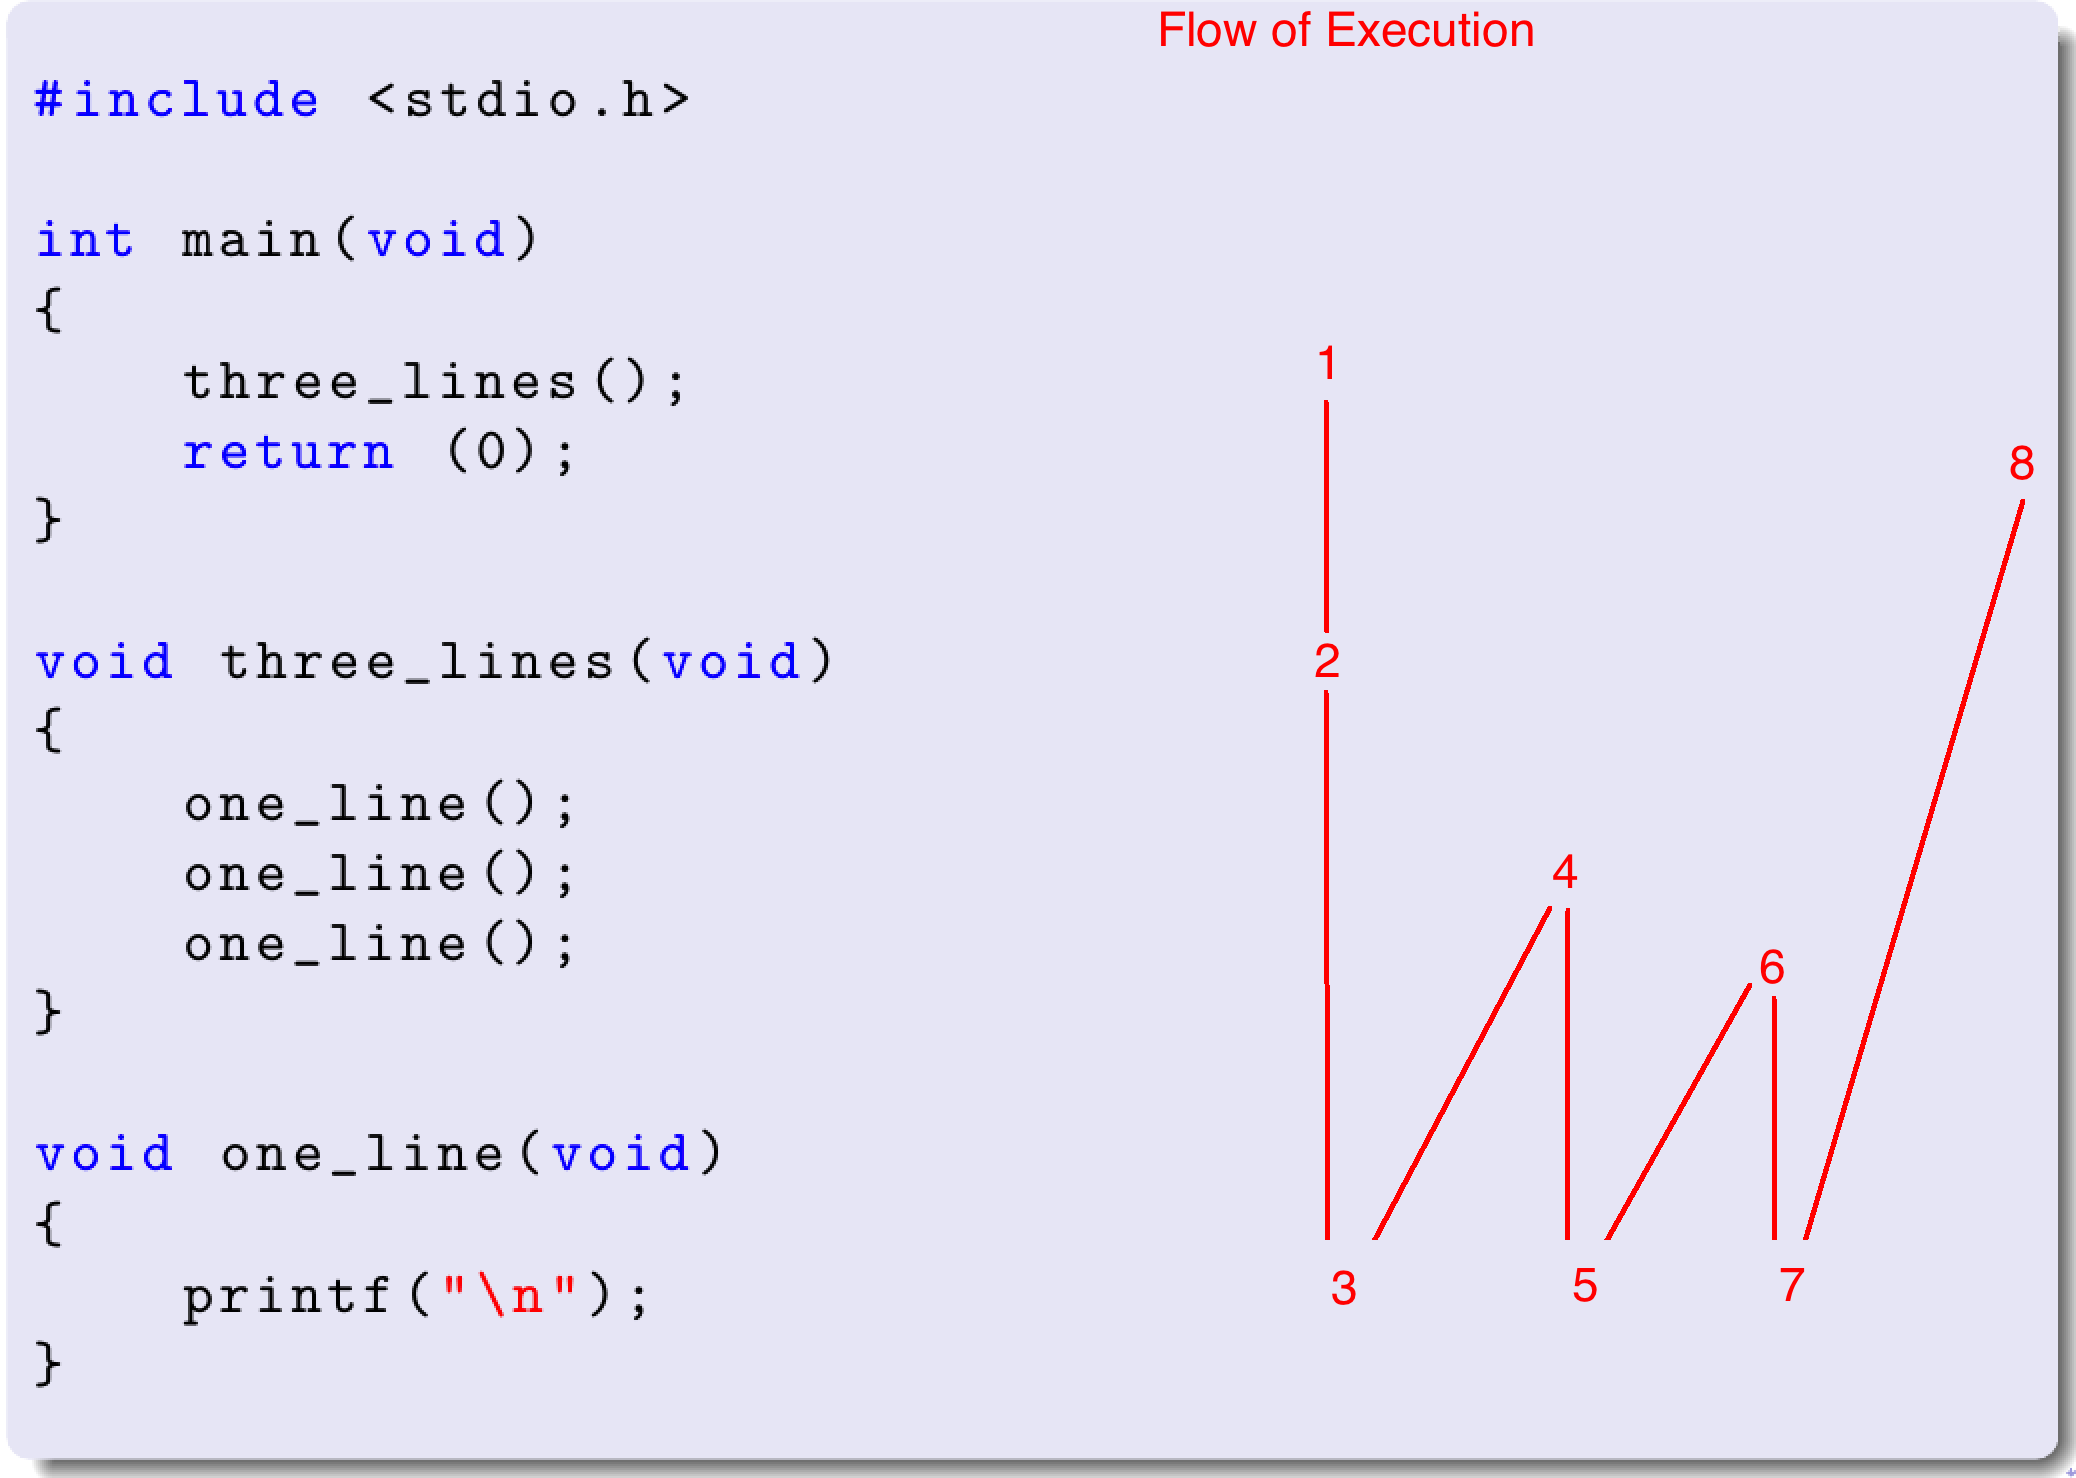
\includegraphics[scale=0.165]{Code1.png}
\end{frame}

\begin{frame}
\textbf{ Flow of Execution}
\begin{itemize}
\item Fortunately, C is adept at keeping track of where it is, 
\item So each time a function completes, 
\item The program picks up where it left off in the function that called it. 
\item When it gets to the end of the program (i.e. the end of the main function)
\item It terminates.
\end{itemize}
\end{frame}

\begin{frame}
\begin{itemize}
\item When you read a program, 
\item don’t read from top to bottom. 
\item Instead, follow the flow of execution. 
\end{itemize}
\end{frame}

\begin{frame}
\begin{itemize}
\item To this point, the functions that we have written
\end{itemize}
\begin{itemize}
\item Cause detours in the flow of execution
\item But take no input as they do so
\item And return no output
\item Though they do print to the \textbf{standard out} (usually the screen)
\end{itemize}
\end{frame}

\begin{frame}
\begin{itemize}
\item As we build more complex functions, we may need to
\end{itemize}
\begin{itemize}
\item Provide input to our functions
\item And have them return values or data
\item Rather than just printing to the screen
\end{itemize}
\end{frame}

\begin{frame}[fragile]
\textbf{Arguments and Parameters}

\begin{itemize}
\item In order to pass data \textbf{to} a function in C, we use a combination of parameters and arguments
\item A parameter is what appears in the definition of the function. 
\item An argument is the instance passed to the function at runtime.
\end{itemize}
\end{frame}

\begin{frame}[fragile]
\begin{block}{}
\begin{lstlisting}
#include <stdio.h>

int main(void) 
{
    print_input(3);
    return 0;
}

void print_input(int i)
{
    printf("%d\n", i);
}
\end{lstlisting}
\end{block}
\end{frame}

\begin{frame}
\textbf{Returning Data from Functions}
\begin{itemize}
\item Just as some of the functions that we write accept input
\item Some (but not all) will also return output
\item In other words you can write functions that yield results. 
\item If you want to pass on the result, you use the 'return'  statement. 
\end{itemize}

\end{frame}

\begin{frame}[fragile]
\begin{block}{}
\begin{lstlisting}
#include <stdio.h>

int main(void) 
{
    int num1 = 7;
    int num2 = 3;
    int result = remainder_of(num1,num2);
    print_input(result);
    return 0;
}

void print_input(int i)
{
    printf("%d\n",i);
}

int remainder_of(int i, int j)
{
    return (i%j);
}
\end{lstlisting}
\end{block}

\end{frame}

\begin{frame}
\textbf{Aside: Modulo}
\begin{itemize}
\item Note the use of the modulo or \% operator in the previous code example
\item The modulo operator works on integers (and integer expressions) 
\item Yields the remainder when the first operand is divided by the second. 
\end{itemize}
\end{frame}

\begin{frame}
\begin{itemize}
\item if x\%y is zero, then x is divisible by y  - e.g. 4\%2 = 0 
\item x \% 10 yields the rightmost digit of x (in base 10) - e.g. 124 \% 10 = 4
\item x \% 100 yields the last two digits - e.g. 124 \% 100 = 24
\end{itemize}
\end{frame}

\begin{frame}
 
\textbf{Back to Functions}
 
\begin{itemize}
\item Note also that there need not be any relationship between
\begin{itemize}
\item passing an input argument and
\item returning a value
\end{itemize}
\item Functions can,
\begin{itemize}
\item pass no argument and return no value
\item pass no argument and return a value
\item pass an argument but return no value
\item pass an argument and return a value 
\end{itemize}
\end{itemize}
\end{frame}

\begin{frame}[fragile]
\begin{itemize}
\item A return statement ends the execution of the function 
\item Control is then passed back to the code that called the function. 
\item Code that appears in a function after a return statement, or any other place, the flow of execution can never reach, is called dead. 
\bigskip
% \item It may surprise you to learn that in C, all functions can contain a return statement, even those marked as void
% \item Return statements in functions marked as void return the flow of control to the calling code but cannot return a value
\end{itemize}
\end{frame}

\begin{frame}[fragile]
\begin{block}{}
\begin{lstlisting}
#include <stdio.h>

int main(void) 
{	
    print_input(remainder_of(2,5));
    return 0;
}

int remainder_of(int i, int j)
{
    return (i%j);
    /* dead code */
    int new_result = (j%i);
    print_input(new_result);
}

void print_input(int i)
{
    printf("%d\n",i);
}
\end{lstlisting}
\end{block}
\end{frame}


\begin{frame}
\begin{itemize}
\item C forces us to define data types at compile time for 

\begin{itemize}
\item Arguments and parameters
\item Return values
\end{itemize}
\item In this sense, C is pretty strict in its handling of types
\end{itemize}
\end{frame}


\begin{frame}
 
\textbf{Terminology : Typed Languages}
 

\begin{itemize}
\item Statically typed language 

\begin{itemize}
\item A language in which types are fixed at compile time
\item Most statically typed languages enforce this by requiring you to declare all variables with their datatypes before using them 
\item C and Java are statically typed languages
\end{itemize}

\item Dynamically typed language 
\begin{itemize}
\item A language in which types are discovered at execution time - the opposite of statically typed
\item JavaScript and Python are dynamically typed, because they figure out what type a variable is when you first assign it a value 
\end{itemize}
\end{itemize}
\end{frame}

\begin{frame}
\begin{itemize}
\item Strongly typed language 

\begin{itemize}
\item A language in which types are always enforced
\item Java and Python are strongly typed. If you have an integer, you can't treat it like a float without explicitly converting it. 
\end{itemize}
\item Weakly typed language 

\begin{itemize}
\item A language in which types may be ignored; the opposite of strongly typed 
\item Perl and VBScript are weakly typed 
\item In VBScript, you can concatenate the string '12' and the integer 3 to get the string '123', then treat that as the integer 123, all without any explicit conversion. 
\end{itemize}
\end{itemize}
\end{frame}

\begin{frame}
\begin{itemize}
\item C (like Java) is

\begin{itemize}
\item Statically typed: because it uses explicit datatype declarations 
\item Strongly typed: because once a variable has a datatype, it actually matters. 
\end{itemize}
\end{itemize}
\end{frame}

\begin{frame}[fragile]
\textbf{Aside: Type Conversion}
\begin{itemize}
\item It is possible in C to convert between types
\item The first is implicit conversion, for example of integers to floats during division
\item This is also called \textbf{type coersion}
\begin{itemize}
\item float x = 9 / 1.0;
\end{itemize}
\item The second is \textbf{casting}, which \textbf{explicitly} changes data of one type  type to data of another
\item for example, casting an integer to a float
\end{itemize}
\begin{block}{}
\begin{lstlisting}
#include <stdio.h>

main() {
   int sum = 17, count = 5;
   double mean;

   mean = (double) sum / count;
   printf("Value of mean : %f\n", mean );
}
\end{lstlisting}
\end{block}
\end{frame}

\begin{frame}
\textbf{Aside: Robustness}
\begin{itemize}
\item You should also note that your code may at some point receive unexpected input 
\begin{itemize}
\item e.g. a parameter of the wrong type (e.g. double instead of int)
\item e.g. a parameter that is out of range (e.g. a negative number when a positive one is expected
\end{itemize}
\item The user might not be aware of this
\item Your code should exit gracefully when wrong input is provided
\item In other words, your code has to be made \textbf{robust}
\item We will look at ways to make your code robust as we progress through the course
\end{itemize}
\end{frame}

\begin{frame}[fragile]
\textbf{Back to Functions}
\begin{itemize}
\item Function variables and parameters are local
\item Variables created \textit{inside} a function can only be used \textit{inside}. 
\item When example\_function terminates in the following code, the value of the variable example\_variable is destroyed. 
\item The following code generates an error at compile time
\end{itemize}
\end{frame}

\begin{frame}[fragile]
\begin{block}{}
\begin{lstlisting}
#include <stdio.h>

int main(void) 
{
    example_function();
    printf("%d\n", example_variable);
    return 0;
}

void example_function()
{
    int example_variable = 4;
    printf("%d\n", example_variable);
}
\end{lstlisting}
\end{block}
\end{frame}

\begin{frame}[fragile]
\begin{itemize}
\item The same rules that apply to variables also apply to parameters 
\item For example, outside the function example\_function2, there is no such thing as example\_param 
\item If you try to use it, C will complain 
\end{itemize}
\end{frame}

\begin{frame}[fragile]
\begin{block}{}
\begin{lstlisting}
#include <stdio.h>

int main(void) 
{
    example_function2();
    printf("%d\n", example_param);
    return 0;
}

void example_function2(int example_param)
{
    int example_variable = 4;
    printf("%d\n", example_variable);
}
\end{lstlisting}
\end{block}
\end{frame}

\begin{frame}[fragile]
\begin{itemize}
\item We can, however, create variables whose scope is not limited (i.e. variables that can be used throughout your code) 
\item Those variables are described as global variables
\item Global variables are (rather unsurprisingly) defined \textit{outside }individual functions 
\end{itemize}
\end{frame}

\begin{frame}[fragile]
\begin{block}{}
\begin{lstlisting}
#include <stdio.h>

int example_global_variable = 3;

int main(void) 
{
    example_function();
    printf("%d\n", example_global_variable);
    return 0;
}

void example_function()
{
    printf("%d\n", example_global_variable);
}

\end{lstlisting}
\end{block}
\end{frame}

\begin{frame}
\begin{itemize}
\item Bringing those two ideas together: 
\bigskip
\item Global variables can be accessed from everywhere 
\item Other variables and parameters can only be accessed within the function where they are defined
\begin{itemize}
\item and can only be accessed after being defined
\end{itemize}
\item The area in which a variable can be referenced is called the \textbf{scope} of the variable 
\item In C, braces define the scope of a variable. 
\bigskip
\item {\itshape Since all of our code sits within the global scope }
\item {\itshape We say that the scope of the function is nested in the global scope }
\end{itemize}
\end{frame}

\begin{frame}
\begin{itemize}
\item The functions we have looked at so far either print to the standard out or return the result of a simple calculation
\item We may not, of course, want to return the same value every time that we call (execute) a function
\item Before considering branches in an example program that will cause \textbf{different} returns, depending on the arguments passed, we will need to consider a new data type - booleans
\end{itemize}
\end{frame}

\begin{frame}
\textbf{Booleans}
\begin{itemize}
\item A boolean can have one of two values
\begin{itemize}
\item true
\item false
\end{itemize}
\end{itemize}
\begin{itemize}
\item You can combine booleans using \textbf{and (\&)}, \textbf{or (I)}, \textbf{not (!)}
\begin{itemize}
\item t=true
\item f=false
\item t \& t $\rightarrow $ \ true
\item f \& t $\rightarrow $ false
\end{itemize}
\end{itemize}
\end{frame}

\begin{frame}
\begin{itemize}
\item In programming languages such as Java and C\#, a boolean is a built in type
\item In C a boolean is not a built in type 
\item (However \textless stdbool.h \textgreater does provide this functionality)
\item In C boolean values (i.e. TRUE and FALSE) are represented as 1 and 0
\end{itemize}
\end{frame}

\begin{frame}

 
\textbf{Comparisons}
 
\begin{itemize}
\item We can compare values or expressions that evaluate to numbers in the following way
\begin{itemize}
\item 3 {\textless} 5 $\rightarrow $ true (1)
\item 3.0 {\textless} 5 $\rightarrow $ true (1)
\item 3!=5 $\rightarrow $ true (1)
\item 3 == 5 $\rightarrow $ false (0)
\item 3 {\textless} 5 {\textless}=7 $\rightarrow $ true (1)
\item 3 {\textless} 5 {\textgreater} 2 $\rightarrow $ true (1)
\end{itemize}
\end{itemize}
\end{frame}

\begin{frame}[fragile]
\textbf{Assignment and Testing}
\begin{itemize}
\item Please note the difference between assignment and testing for equality
\begin{itemize}
\item Use a single equals sign (=) for assignment
\item Use a double equals sign (==) to test if two things have equal values 
\end{itemize}
\end{itemize}
\end{frame}

\begin{frame}[fragile]
\begin{block}{}
\begin{lstlisting}
#include <stdio.h>

int main(void) 
{
    int x = 5;
    
    printf("%d\n", (5 == x));
    
    printf("%d\n", (x == 4));
    
    return 0;
}
\end{lstlisting}
\end{block}
\end{frame}

\begin{frame}[fragile]
 
\textbf{Conditional Statements}
 
\begin{itemize}
\item Armed with boolean statements, we can go on to create \textbf{conditional statements} in our code
\item Conditional statements allow us to check certain conditions and change the behaviour of the program accordingly
\item The simplest conditional statement is the if statement (also described as the IF-THEN statement)
\end{itemize}

\begin{block}{}
\begin{lstlisting}
if (testscore >= 90) 
{
   char grade = 'A';
}
\end{lstlisting}
\end{block}
\end{frame}


\begin{frame}
\begin{itemize}
\item The example on the previous slide uses conditional control statements (e.g. an if statement) to create conditional branching, 
\item So called because because this type of control structure causes the flow of execution to branch off in different
directions.
\end{itemize}
\end{frame}

\begin{frame}
\textbf{if statements:}
\begin{itemize}
\item The code between the brackets () is called the condition 
\begin{itemize}
\item If it is 1 (or true), the code between the braces \{\} is executed
\end{itemize}
\item If not (i.e. 0 or false), nothing happens (the indented code is skipped)
\item The condition can be any expression that evaluates to a boolean

\begin{itemize}
\item boolean expressions
\item comparisons
\item functions with booleans as a return value 
\end{itemize}
\end{itemize}
\end{frame}

\begin{frame}
\textbf{Constructing an if statement}
\begin{itemize}
\item if statements, (somewhat) like function definitions are compound statements
\item Their syntax is as follows:
\begin{itemize}
\item if (condition) \{
\begin{itemize}
\item First Statement
\item Second Statement
\item Etc.
\end{itemize}
\item \}
\end{itemize}
\item All the statements between braces are treated as a unit
\item Either all are executed or none
\end{itemize}
\end{frame}

\begin{frame}[fragile]
\begin{itemize}
\item A second form of the if statement is IF/ELSE
\item The else block allows us to provide code that will execute if and only if the condition is NOT met
\end{itemize}
\begin{block}{}
\begin{lstlisting}
if (testscore >= 90) 
{
    grade = 'A';
} 
else
{
    grade = 'B';
}
\end{lstlisting}
\end{block}
\end{frame}

\begin{frame}[fragile]
\begin{itemize}
\item We can chain if/else statements
\end{itemize}

\begin{block}{}
\begin{lstlisting}
if (testscore >= 90) 
{
    grade = 'A';
} 
else if (testscore >= 80) 
{
    grade = 'B';
}
else
{
    grade = 'C';
}
\end{lstlisting}
\end{block}
\end{frame}

\begin{frame}[fragile]

\begin{itemize}
\item We can also nest if/else statements within each other 
\item Note that nesting if/else statements has a different effect to chaining
\end{itemize}

\begin{block}{}
\begin{lstlisting}
int age = 29;
if (age < 16)
{
  printf("Child");
}
else
{
  if (age < 65)
  {
    printf("Adult");
  }
  else
  {
    printf("Senior");
  }
}
\end{lstlisting}
\end{block}
\end{frame}

\begin{frame}[fragile]
\begin{itemize}
\item If you create a function that requires a return statement
\item then you have to guarantee that every possible path through the program hits such a return 
\end{itemize}

\begin{block}{}
\begin{lstlisting}
if (age > 16) 
{
    return "Can drive";
} 
else if (age < 16)
{
    return "Can't drive";
}
\end{lstlisting}
\end{block}
\begin{itemize}
\item PROBLEM: What happens if age = 16?
\end{itemize}
\end{frame}

\begin{frame}
 
\textbf{Recursion}
 
\begin{itemize}
\item Functions, besides calling other functions, can also call themselves.
\item This turns out to be rather useful.
\item The process of a function calling itself is called \textbf{recursion} 
\item functions which perform recursion are said to be \textbf{recursive} 
\end{itemize}
\end{frame}


\begin{frame}[fragile]
\begin{itemize}
\item This code will count down from n (try it in the lab) 
\item It will, however, attempt to keep going indefinitely (and eventually crash)
\end{itemize}

\begin{block}{}
\begin{lstlisting}
#include <stdio.h>

int main(void) {
    example_recursive_function(5);
    return 0;
}

void example_recursive_function(int counter)
{
    printf("%d\n",counter);
    example_recursive_function(counter-1);
}
\end{lstlisting}
\end{block}
\end{frame}

\begin{frame}
 
\textbf{Recursion Problem Specification}
 
\begin{itemize}
\item Recursive problems (and correctly constructed recursive functions) have at least one simple case, \textbf{the base case}, which can be solved without recursion
\item All other cases can be reduced to a case closer to the base case by means of recursion\newline
\item Eventually all cases can be reduced to the base case 
\item If recursion never reaches a base case it will continue making recursive calls forever.
\item This is called infinite recursion. 
\item A finite amount of memory is consumed on each recursive call, and eventually the program will terminate with an error
\end{itemize}
\end{frame}

\begin{frame}

\begin{itemize}
\item {\bfseries Recursion: Structure}

\begin{itemize}
\item IF the base case is reached 

\begin{itemize}
\item SOLVE
\end{itemize}
\item ELSE

\begin{itemize}
\item reduce the problem using recursion
\end{itemize}
\end{itemize}
\item {\bfseries Definition: Problem Size}

\begin{itemize}
\item The number of reduction steps a problem is away from the base case is the \textbf{problem size}
\end{itemize}
\bigskip
\item The following code counts down to zero and then stops (assuming positive input)
\end{itemize}
\end{frame}

\begin{frame}[fragile]
\begin{block}{}
\begin{lstlisting}
#include <stdio.h>

int main(void) {
    example_recursive_function(5);
    return 0;
}

void example_recursive_function(int counter)
{ 
   if(counter == 0)
   {
       return;
   }
   else 
   {
       printf("%d\n",counter);
       example_recursive_function(counter-1);
   }

}

\end{lstlisting}
\end{block}
\end{frame}


\begin{frame}
\begin{itemize}
\item the if-statement (if counter == 0) contains the base case criteria
\item If we reach this case, we can stop the recursive calling of the function or print or return the result
\item The else-statement prints the current counter 
\item And then calls the example\_recursive\_function function with the lower counter value 
\end{itemize}
\end{frame}

\begin{frame}[fragile]
\begin{itemize}
\item This output from this code is as follows:

\begin{block}{}
\begin{lstlisting}
$ gcc -o example example.c

$ ./example
5
4
3
2
1

\end{lstlisting}
\end{block}
\end{itemize}
\end{frame}

\begin{frame}
\textbf{Stacks}
\begin{itemize}
\item You should note that taking a recursive approach to problems that require a great number of steps to reach the base case (have a large problem size) places a heavy burden on computer memory
\end{itemize}
\end{frame}

\begin{frame}
\textbf{Stacks}
\begin{itemize}
\item C uses a ``stack'' to store the data held in variables as code executes 
\item A stack can be seen as a pile of plates. 
\item Clean (new) plates go on top 
\item And plates are always taken from to top. 
\item So a stack works: LIFO:
\begin{itemize}
\item Last In First Out 
\end{itemize}
\item These ``Plates'' are referred to as \textbf{frames}
\end{itemize}
\end{frame}

\begin{frame}
\begin{itemize}
\item Every time you call a function or a procedure, 
\item memory is allocated on the memory stack to store the parameters and local variables
\item As the following example shows, those parameters and variables are stored {}``above'' those that went before 
\item This means that they will be accessed before those that went before
\end{itemize}
\end{frame}

\begin{frame}
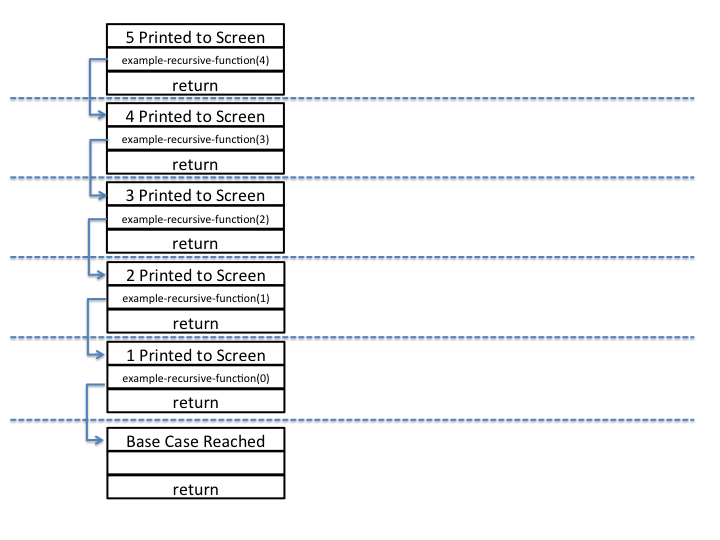
\includegraphics[scale=0.5]{Slide2.png}
\end{frame}

\begin{frame}
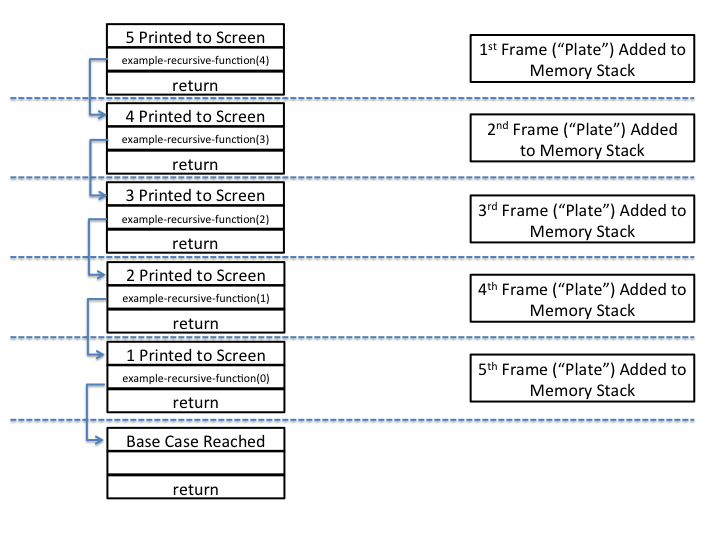
\includegraphics[scale=0.5]{Slide3.png}
\end{frame}

\begin{frame}
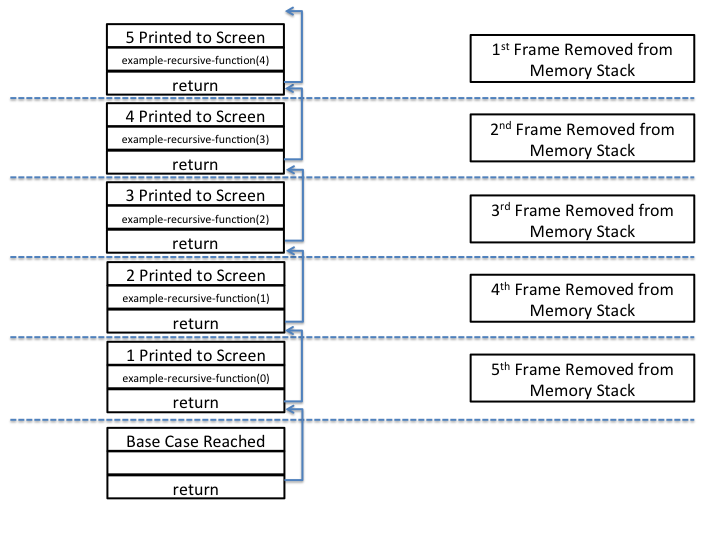
\includegraphics[scale=0.5]{Slide4.png}
\end{frame}

\begin{frame}
 
\textbf{Fibonacci Sequence}
 
\begin{itemize}
\item The first lab sheet asked you to write code that calculates the first n numbers in the Fibonacci sequence 
\item We will now consider a recursive programming approach to that problem
\end{itemize}
\end{frame}

\begin{frame}
 
\textbf{Fibonacci Sequence}
 
\begin{itemize}
\item Problem Definition: number n in the Fibonacci sequence is the sum of numbers (n-1) and (n-2) in that same sequence
\item The first three numbers in the sequence are 0, 1 and 1
\end{itemize}
\end{frame}

\begin{frame}
 
\textbf{Fibonacci Sequence : Pseudocode}
 
\begin{itemize}
\item In pairs (or threes) write this algorithm in pseudocode
\bigskip
\item HINT: The first 7 numbers in the Fibonacci sequence are 
\item 0  1  1  2  3  5  8
\end{itemize}
\end{frame}

\begin{frame}[fragile]
\begin{block}{}
\begin{lstlisting}
int fibonacci(int n)
{ 
   if(n == 0)
   {
      return 0;
   }
   else if(n == 1)
   {
      return 1;
   }
   else
   {
      return fibonacci(n - 1) + fibonacci(n - 2);
   }

}
\end{lstlisting}
\end{block}

\end{frame}

\begin{frame}[fragile]
\begin{itemize}
\item In pairs (or threes) try to write down the rise and fall of the memory stack in this code...
\end{itemize}
\end{frame}

\end{document}

